 
\resizebox{.7\textwidth}{.35\textheight}{
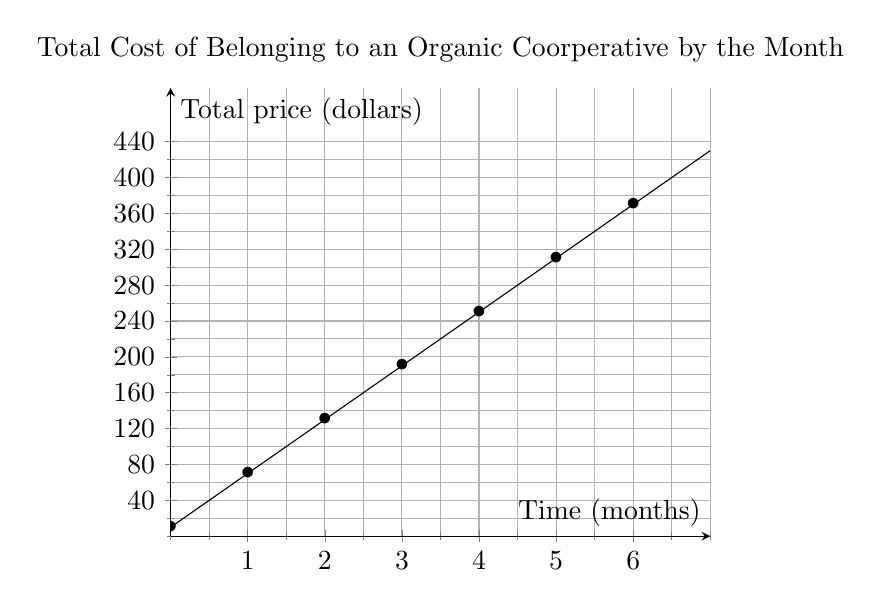
\begin{tikzpicture}
\begin{axis}[xmin=0,ymin=0,xmax=7, ymax=500, xtick={0,1,2,3,4,5,6}, ytick={0,40,80,120,160,200,240,280,320,360,400,440},axis lines=center,
ylabel= {Total price (dollars)}, xlabel={Time (months)}, title={Total Cost of Belonging to an Organic Coorperative by the Month},grid=minor, grid style={solid, black!30!white,},minor xtick={0,.5,...,7}, minor ytick = {0,20,40,...,440},]
\addplot[samples=17,domain=0:7,]{60*x+10};
\draw (axis cs: 0,10)node{$\bullet$} (axis cs:1,70)node{$\bullet$} 
(axis cs: 2,130)node{$\bullet$} (axis cs: 3,190)node{$\bullet$}
(axis cs: 4,250)node{$\bullet$} (axis cs: 5, 310)node{$\bullet$}
(axis cs: 6,370)node{$\bullet$}; 
\end{axis}
\end{tikzpicture}}\\
The graph above displays the total price $p$ paid by a customer to belong to an organic cooperative for $m$ months.  What does the slope represent in the graph?



\ifsat
	\begin{enumerate}[label=\Alph*)]
		\item The initial cost of joining the cooperative.
		\item The total number of months spent with the cooperative.
		\item The total number of organic products purchased via the cooperative.
		\item The increase in cost to stay with the cooperative for each additional month. % 
	\end{enumerate}
\else
\fi

\ifacteven
	\begin{enumerate}[label=\textbf{\Alph*.},itemsep=\fill,align=left]
		\setcounter{enumii}{5}
		\item The initial cost of joining the cooperative.
		\item The total number of months spent with the cooperative.
		\item The total number of organic products purchased via the cooperative.
		\addtocounter{enumii}{1}
		\item The increase in cost to stay with the cooperative for each additional month. % 
		\item None of these. 
	\end{enumerate}
\else
\fi

\ifactodd
	\begin{enumerate}[label=\textbf{\Alph*.},itemsep=\fill,align=left]
		\item The initial cost of joining the cooperative.
		\item The total number of months spent with the cooperative.
		\item The total number of organic products purchased via the cooperative.
		\item The increase in cost to stay with the cooperative for each additional month. % 
		\item None of these. 
	\end{enumerate}
\else
\fi

\ifgridin
 The increase in cost to stay with the cooperative for each additional month. % 

\else
\fi

